\documentclass{standalone}
\usepackage{tikz}
\usetikzlibrary{automata, positioning}

\begin{document}
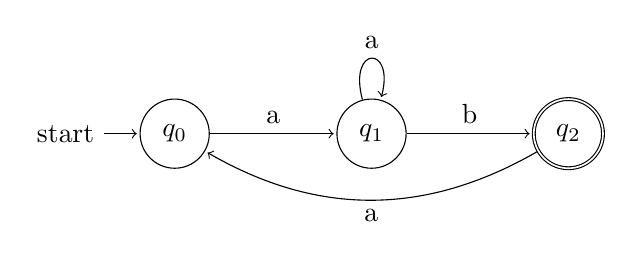
\begin{tikzpicture}[shorten >=1pt,node distance=2.5cm,on grid,auto]
    % Define the states
    \node[state,initial] (q0) {$q_0$}; 
    \node[state] (q1) [right=of q0] {$q_1$};
    \node[state,accepting] (q2) [right=of q1] {$q_2$};

    % Draw transitions
    \path[->] 
        (q0) edge node {a} (q1)
        (q1) edge [loop above] node {a} ()
        (q1) edge node {b} (q2)
        (q2) edge [bend left] node {a} (q0);
\end{tikzpicture}
\end{document}